\documentclass[a4paper]{article}

\usepackage{xcolor}
\usepackage{fancyhdr}
\usepackage{listings}
\usepackage{graphicx}
\usepackage[utf8]{inputenc}
\usepackage{multirow}
\lstset{frameround=fttt,numbers=left,breaklines=true, extendedchars=true}

\newcommand{\todo}[1]{\textcolor{red}{[#1]}}
\lhead{Open Universiteit}
\chead{IM0202, Software evolution}
\rhead{Assignment 2}

\begin{document}
\pagestyle{fancy}

\section*{Studentgegevens}
\begin{description}
	\item [Cursuscode]: IM0202
	\item [Naam]: Ewoud Westerbaan
	\item [Studentnummer]: 852069942
	\item [Naam]: Martin de Boer
	\item [Studentnummer]: 837372832
\end{description}

\section{Samenwerking}
De eerste iteratie is gebouwd op basis van een experiment van Martin, die tijdens de kerstdagen al was begonnen. Deze uitkomst hebben we als basis genomen en bepaald wat toegevoegd en / of aangepast zou moeten worden. Vooral Martin heeft hier veel werk in verzet.
Het cache mechanisme en een eerste versie van een zelfgemaakte boxplot is door Ewoud gemaakt, maar deze boxplot is later door Martin nog iets verbeterd. Rascal biedt nog geen boxplot aan (deze is nog in experimentele fase).


\section{Aannames}
\begin{description}
\item[Data is consistent] We gaan ervan uit dat de data waar de visualisatie op maken, dezelfde is als de data uit assignment 1. Voor de visualisatie gebruiken we niet de duplicatiemetrieken.
\item[Kleurenblindheid en grijstinten] De visualisatie is niet gemaakt voor mensen met kleurenblindheid of voor het afdrukken in grijstinten.
\end{description}

\section{Criteria}
Criteria met betrekking tot esthetiek en gebruiksvriendelijkheid:
\begin{enumerate}
\item Voorkom vertekeningen in waarnemingen \cite{tufte2014visual} p.56. Hiermee wordt bedoeld dat de fysieke grootte van een object in verhouding moet staan met de werkelijke numerieke waarde. Een verkeerde verhouding noemt Tufte de `Lie Factor'.
\item Aantal informatie dragende dimensies mag niet groter zijn dan het aantal dimensies in de data \cite{tufte2014visual} p.71. Tufte geeft aan dat het gebruik van meerdere dimensies ten opzichte van het aantal dimensies dat de data bevat, leidt tot misleiding en fouten in het ontwerp.

\item Stephen Few geeft enkele criteria met betrekking tot kleurgebruik \cite{B}:
\begin{enumerate}
\item Gebruik zachte kleuren, tenzij je iets uit wilt lichten;
\item Gebruik dezelfde kleur, tenzij dit geassocieerd wordt met een andere betekenis; 
\item Gebruik een enkele, neutrale achtergrond kleur.
\end{enumerate}

\item Ben Shneiderman heeft voor gebruiksvriendelijkheid de `Visual Information-Seeking Mantra` beschreven. Deze theorie houdt in dat eerst een overzicht gegeven moet worden, vervolgens men moet kunnen inzoomen en filteren. Details moeten op aanvraag beschikbaar zijn \cite{A}. Tufte geeft ook een zelfde principe: `reveal the data at several levels of detail, from a broad overview to the fine structure` \cite{tufte2014visual} p. 13.
\end{enumerate}


\section{Selectie van de architectural view}
Het doel van onze visualisatie is de kwaliteit van een applicatie op basis van complexiteit en unitsize te laten zien voor ontwikkelaars in een nieuwbouw- of beheerfunctie. In Figuur \ref{fig:overview} is een overzicht van de visualisatie te zien.

\begin{figure}[h]
  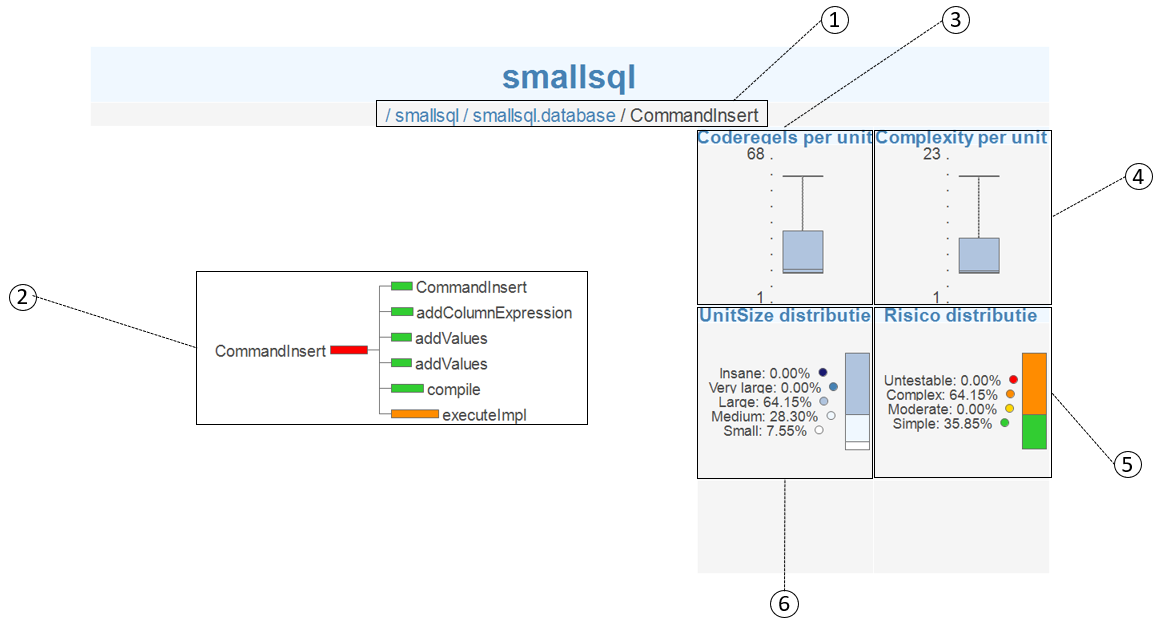
\includegraphics[width=\linewidth]{images/overview_with_numbers.png}
  \caption{Overview}
  \label{fig:overview}
\end{figure}

Het grootste deel van het scherm bestaat uit een treeview. We hebben voor een treeview gekozen, omdat we daar meerdere metrieken in kwijt kunnen; de complexiteitwaarde wordt getoond in kleur, unitsize in grootte, en de hiërarchie van de applicatie doormiddel van de structuur van de figuur (Figuur \ref{fig:overview}: \textcircled{2}). Om het overzicht te bewaren, laat de treeview niet direct waardes zien, maar zijn deze in een popup van een element (package, klasse of methode) te zien wanneer men met de muis hier overheen gaat, zie Figuur \ref{fig:treeview_popup}. Interactiviteit is ingebouwd op de volgende manieren: 1) men kan inzoomen door op een klasse of package te klikken 2) men kan uitzoomen door een shift+klik te doen op een parent node. Het meest gedetailleerde niveau is een methode of constructor.

\begin{figure}[h]
  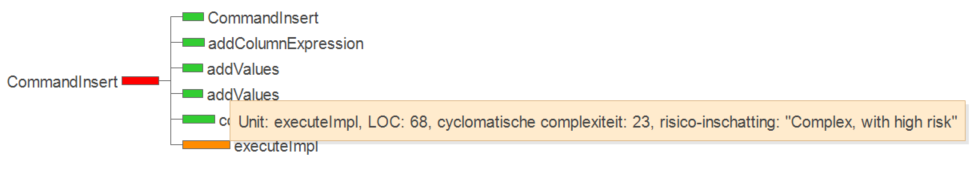
\includegraphics[width=\linewidth]{images/treeview_with_popup.png}
  \caption{Treeview met popup}
  \label{fig:treeview_popup}
\end{figure}

Om een overzicht te geven waar men zich in de hiërarchie van de applicatie bevindt, wordt een kruimelpad getoond (Figuur \ref{fig:overview}: \textcircled{1}). Men kan uitzoomen door op het gewenst niveau te klikken. De klikbare delen hebben een andere kleur (blauw) dan niet-klikbare delen (zwart).
\begin{figure}[ht]
\centering
  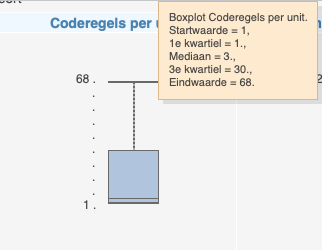
\includegraphics{images/boxplot_popup.png}
  \caption{Boxplot met popup}
  \label{fig:boxplot_popup}
\end{figure}


De zijkant bevat een paneel met inzicht in de verdeling van waardes. Een stackedbar biedt inzicht in de verhouding van de classificaties in het geselecteerde niveau. Naast deze stackedbar zijn de percentages zichtbaar. Een boxplot geeft de verdeling van waardes. Een mouse-over laat een popup zien van de waardes (minimum, 1e kwartiel, mediaan, 3e kwartiel en maximum), zie Figuur \ref{fig:boxplot_popup}.
Een stacked bar en boxplot worden getoond voor complexiteit en unitsize (Figuur \ref{fig:overview}: \textcircled{3}\textcircled{4}\textcircled{5}\textcircled{6}).


\section{Resultaten analyse}
Het voorkomen van vertekeningen hebben we minder goed toegepast. De grootte van de boxes in de treeview zijn hier een voorbeeld van, zo ook de punten aan de zijkant van de boxplot, dit zijn er altijd 10 en dat kan misleidend zijn.

Het aantal informatie dragende dimensies hebben we wel goed toegepast. De boxplotten en stackedbars zijn een 1-dimensionale weergave van een metriek. In de treeview worden twee dimensies weergegeven doormiddel van kleur en grootte. 

De kleurstelling die we hebben toegepast is in de gehele visualisatie hetzelfde. Veel neutraal blauw. De achtergrond hebben we een neutrale lichte kleur gegeven. De achtergrond aan de zijkant waar de boxplotten en stapelboxen staan, hebben we wel een andere kleur gegeven die iets donkerder is, maar nog steeds neutraal. Doordat dit een andere kleur is, associeert men hier een andere betekenis mee, wat in dit geval dus een detaillering is die in het eerste gezicht niet nodig is. Wij willen hiermee bereiken dat men eerst geleid wordt naar de treeview, anders zou de gehele visualisatie te overweldigend over kunnen komen.

De `Visual Information-Seeking Mantra' hebben we toegepast door de visualisatie te laten starten op project niveau. Door te klikken kan men een niveau inzoomen naar package en/ of klasse niveau. Dit is dan ook de hiërarchie die verwerkt is in de visualisatie. Het op aanvraag beschikbaar zijn van de details zit verwerkt in de visualisatie door alleen de waardes te geven van een metriek, wanneer men met de muis over een boxplot van een metriek gaat (popup), dit geldt ook voor details in de treeview.

\bibliographystyle{abbrv}
\bibliography{verslag_assignment2}

\end{document}
